\begin{homeworkProblem}

\textbf{Normal-Normal Conjugacy:} Implement a Metropolis-Hastings algorithm to find the posterior mean and variance of $\theta$ after observing the value of $Y=y$. The parameter setting: $y=3, \mu=0, \sigma^2=1, \tau^2=4$, and $d=0.1,0.5,1,5,10,100$.

\solution

Let $Y|\Theta=\theta\sim\N(\theta,\sigma^2)$, where $\sigma^2$ is known but $\theta$ is unknown, and its prior is $\theta\sim\N(\mu,\tau^2)$. We can get the posterior distribution of $\theta$ with the Normal-Normal conjugate:
\begin{align*}
\Theta|Y=y &\sim \N\left(\dfrac{\frac{1}{\sigma^2}}{\frac{1}{\sigma^2}+\frac{1}{\tau^2}}y+\dfrac{\frac{1}{\tau^2}}{\frac{1}{\sigma^2}+\frac{1}{\tau^2}}\mu, \dfrac{1}{\frac{1}{\sigma^2}+\frac{1}{\tau^2}}\right) \\
f_{\Theta|Y}(\theta|Y=y) &\propto f_{Y|\Theta}(y|\theta)(y|\theta)\cdot f_{\Theta}(\theta) \propto e^{-\frac{1}{2\sigma^2}(y-\theta)^2}\cdot e^{-\frac{1}{2\tau^2}(\theta-\mu)^2}
\end{align*}
Then we can apply the Random Walk Metropolis: \\
For the state $x$, generate the new state $x'=x+d\cdot\N(0,1)$. Since $\N(0,1)$ is systemic, thus
$$x=x'-d\cdot\N(0,1)\sim x'+d\cdot\N(0,1)$$
which means that the one-step transition probability density has the property $f(x,x')=f(x',x)$. \\
The acceptance rate is
$$a_{x,x'}=\min\left(\dfrac{\pi_{x'}f_{x',x}}{\pi_{x}f_{x,x'}},1\right)=\min\left(\dfrac{\pi_{x'}}{\pi_{x}},1\right)=\min\left(e^{-\frac{1}{2\sigma^2}(y-x')^2-\frac{1}{2\tau^2}(x'-\mu)^2 +\frac{1}{2\sigma^2}(y-x)^2+\frac{1}{2\tau^2}(x-\mu)^2},1\right)$$
And the simulated results are as follows:
\begin{figure}[h]
    \centering
    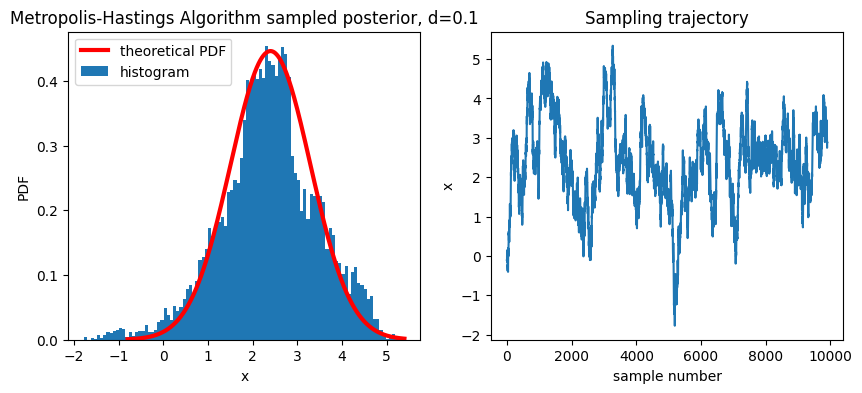
\includegraphics[width=0.49\textwidth]{./figure/p6/0.1.png}
    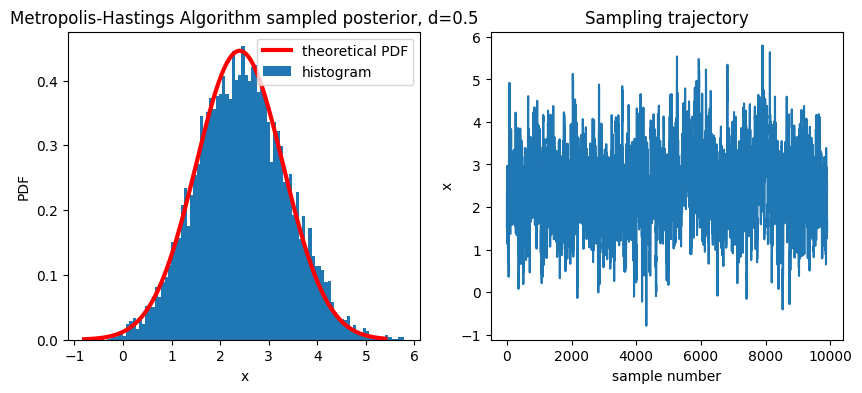
\includegraphics[width=0.49\textwidth]{./figure/p6/0.5.png}
    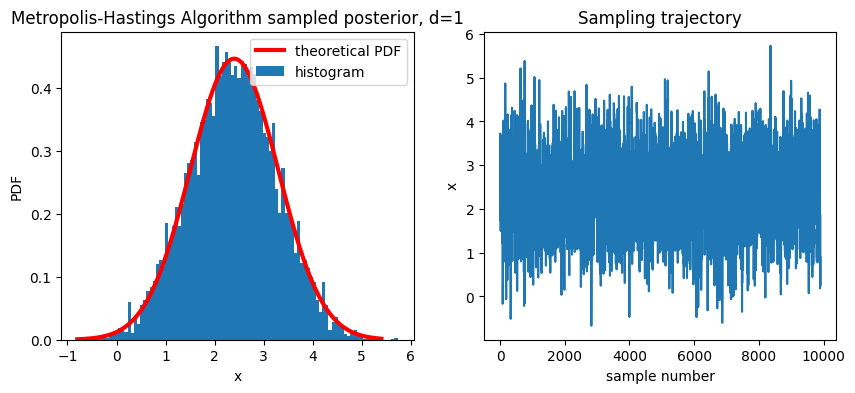
\includegraphics[width=0.49\textwidth]{./figure/p6/1.png}
    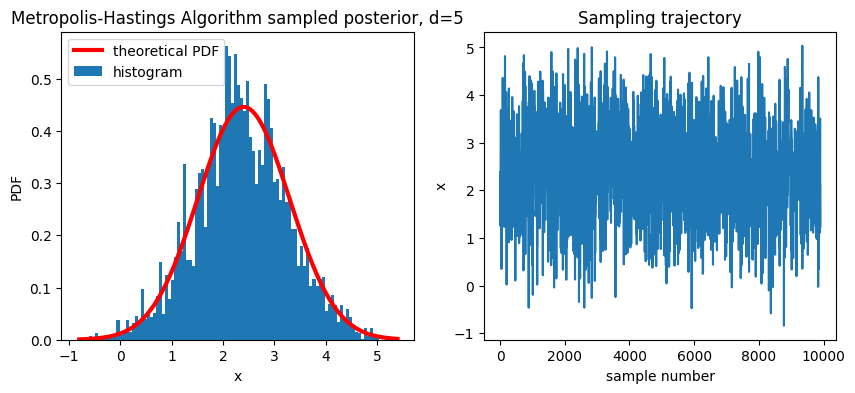
\includegraphics[width=0.49\textwidth]{./figure/p6/5.png}
    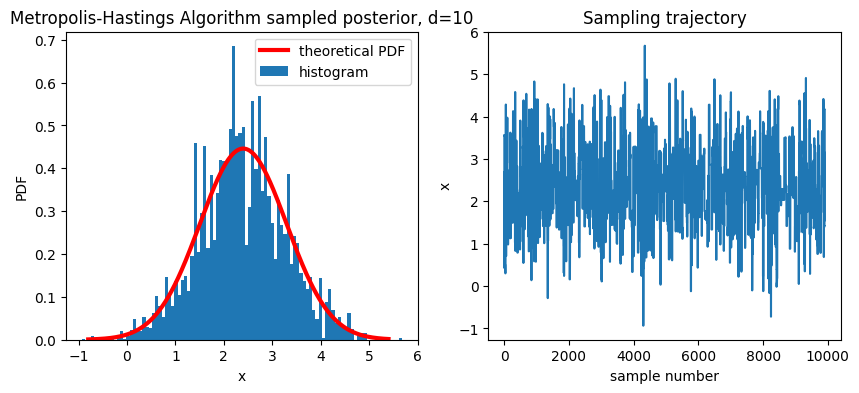
\includegraphics[width=0.49\textwidth]{./figure/p6/10.png}
    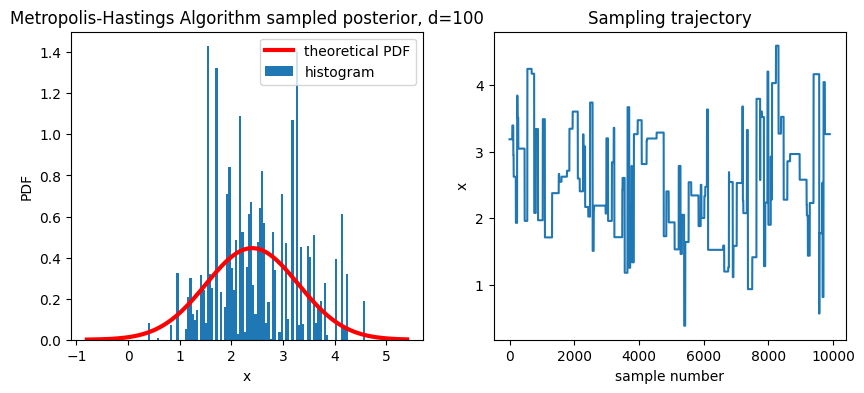
\includegraphics[width=0.49\textwidth]{./figure/p6/100.png}
\end{figure}
When $d$ is too small, the exploration is not enough, causing the restricted mobility. And when $d$ is too large, there are many flatten regions, which means the acceptance rate is too small. So the optimal choice is $d=1$.

And the estimated mean and variance of different $d$ are as follows:
\begin{table}[h]
    \centering
    \begin{tabular}{c cccccc}
    \toprule
    d & 0.1 & 0.5 & 1 & 5 & 10 & 100 \\
    \midrule
    \textbf{mean}     & 2.376 & 2.454 & 2.377 & 2.355 & 2.382 & 2.521 \\
    \textbf{variance} & 1.149 & 0.869 & 0.806 & 0.797 & 0.794 & 0.701 \\
    \bottomrule
    \end{tabular}
\end{table}

The theoritical mean is $2.4$, and variance is $0.8$. From the estimated mean and variance, we could also discover that $d=1$ is the optimal choice.

\end{homeworkProblem}

\newpage